% !TeX root = main.tex
\section*{Results and discussion}

To find a good optimum for the exposure time, a checkerboard pattern is compared for each sample.\todo[inline]{'compared for'???} Optical microscope images of the samples with positive tone and with exposure times coming close to an optimum are shown  below in figures \ref{fig:b3d1}, \ref{fig:b3a1} and \ref{fig:b3e1}.

With the limited amount of developed samples, an exposure time of 2 minutes was found to be optimal. Several images of the positive tone sample with an exposure time of 2 minutes were taken with a Hitachi S4800 scanning electron microscope. These are shown in figures \ref{fig:b2d5_q5}-\ref{fig:b2d10_q11}:

%\begin{figure}[H]
%	\centering
%	\resizebox{\linewidth}{!}{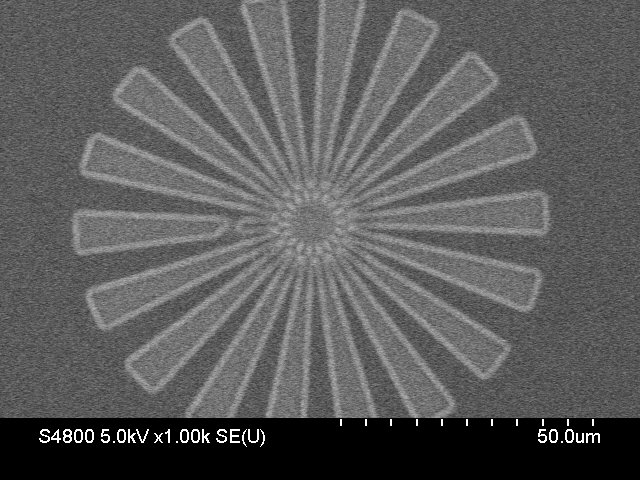
\includegraphics{data/sem/b3a1_q01.jpg}}
%	\caption{SEM}
%	\label{fig:b2d1_q1}
%\end{figure}
%\begin{figure}[H]
%	\centering
%	\resizebox{\linewidth}{!}{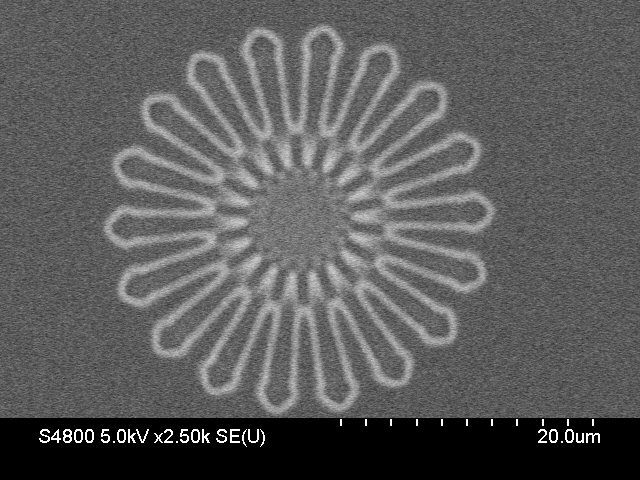
\includegraphics{data/sem/b3a2_q02.jpg}}
%	\caption{SEM}
%	\label{fig:b2d2_q2}
%\end{figure}
%\begin{figure}[H]
%	\centering
%	\resizebox{\linewidth}{!}{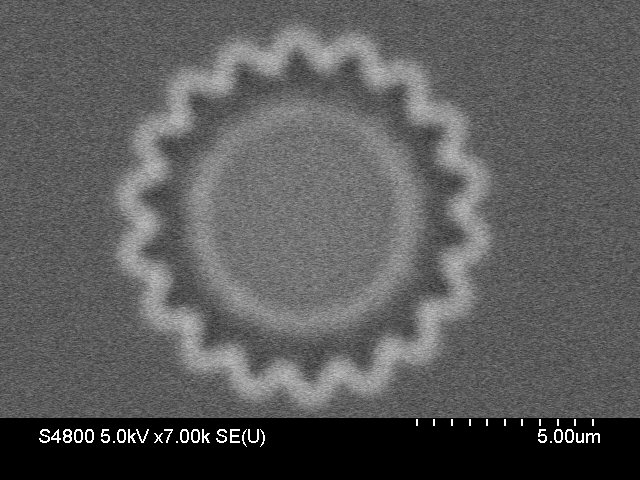
\includegraphics{data/sem/b3a3_q03.jpg}}
%	\caption{SEM}
%	\label{fig:b2d3_q3}
%\end{figure}
\begin{figure*}[ht]
\centering
%    \begin{subfigure}[t]{0.3\linewidth}
%	\centering
%	\resizebox{\linewidth}{!}{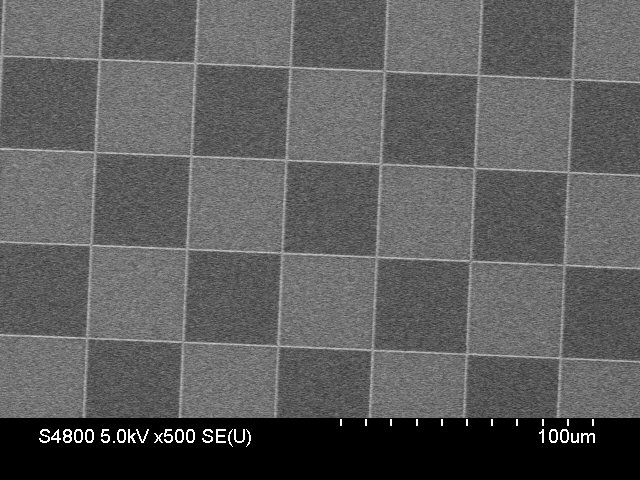
\includegraphics{data/sem/b3a4_q04.jpg}}
%	\caption{Structure size of $\sim$32 $\mu$m.}
%	\label{fig:b2d4_q4}
%\end{subfigure}
    \begin{subfigure}[t]{0.24\linewidth}
	\centering
	\resizebox{\linewidth}{!}{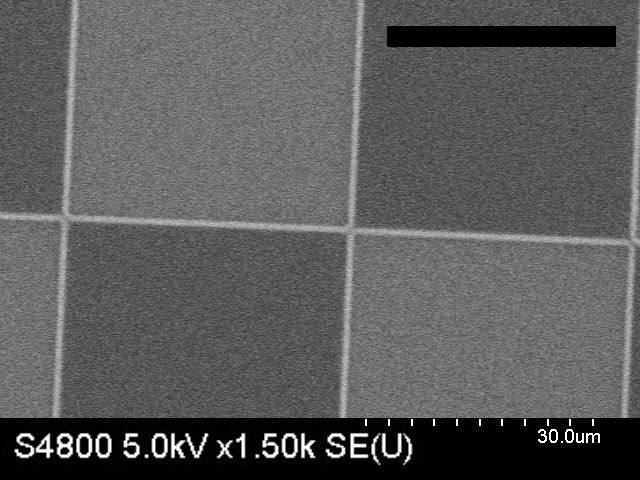
\includegraphics{data/sem/b3a5_q05.jpg}}
	\caption{Structure size of $\sim$35}
	\label{fig:b2d5_q5}
\end{subfigure}
\hfill
% \hspace*{5mm}
%    \begin{subfigure}[t]{0.3\linewidth}
%	\centering
%	\resizebox{\linewidth}{!}{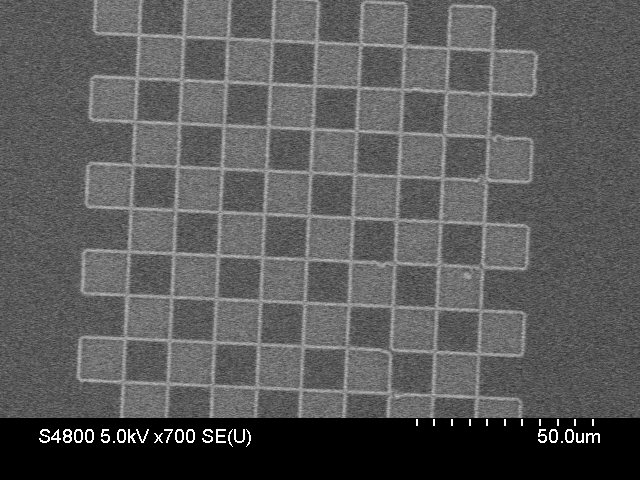
\includegraphics{data/sem/b3a6_q06.jpg}}
%	\caption{Structure size of $\sim$10 $\mu$m.}
%	\label{fig:b2d6_q6}
%\end{figure}
    \begin{subfigure}[t]{0.24\linewidth}
	\centering
	\resizebox{\linewidth}{!}{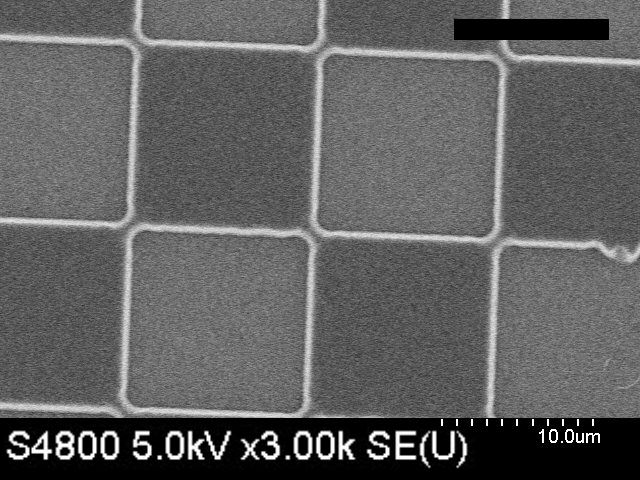
\includegraphics{data/sem/b3a7_q07.jpg}}
	\caption{Structure size of $\sim$10 $\mu$m. Slight overexposure can be seen at the vertices of the squares.}
	\label{fig:b2d7_q7}
\end{subfigure}
%\begin{figure}[H]
%	\centering
%	\resizebox{\linewidth}{!}{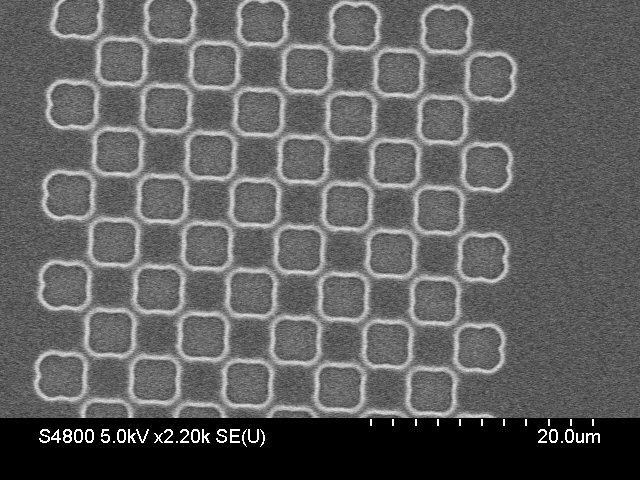
\includegraphics{data/sem/b3a8_q08.jpg}}
%	\caption{Structure size of $\sim$3 $\mu$m.}
%	\label{fig:b2d8_q8}
%\end{figure}
% \\
\hfill
    \begin{subfigure}[t]{0.24\linewidth}
	\centering
	\resizebox{\linewidth}{!}{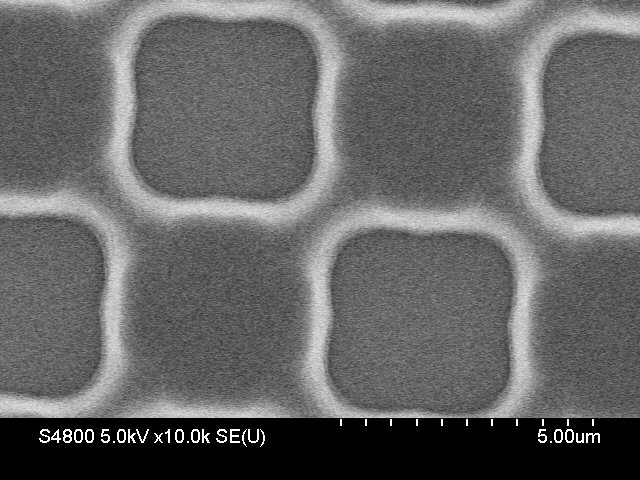
\includegraphics{data/sem/b3a9_q09.jpg}}
	\caption{Structure size of $\sim$4 $\mu$m. The effects of overexposure become pronounced at structure sizes of $\sim$4 $\mu$m.}
	\label{fig:b2d9_q9}
\end{subfigure}
%\begin{figure}[H]
%	\centering
%	\resizebox{\linewidth}{!}{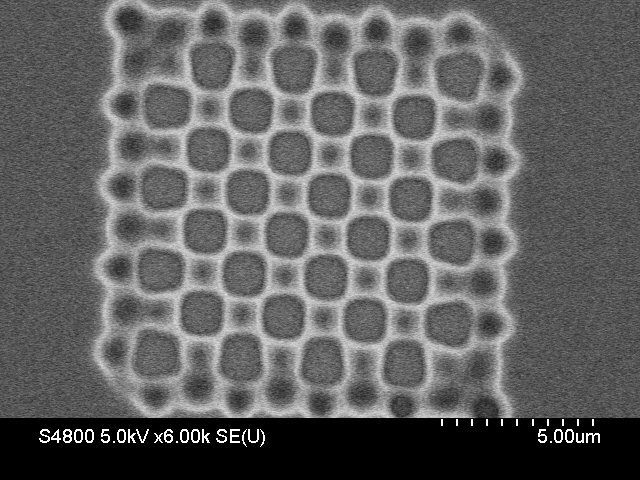
\includegraphics{data/sem/b3a10_q10.jpg}}
%	\caption{SEM}
%	\label{fig:b2d10_q10}
%\end{figure}
\hfill
    \begin{subfigure}[t]{0.24\linewidth}
	\centering
	\resizebox{\linewidth}{!}{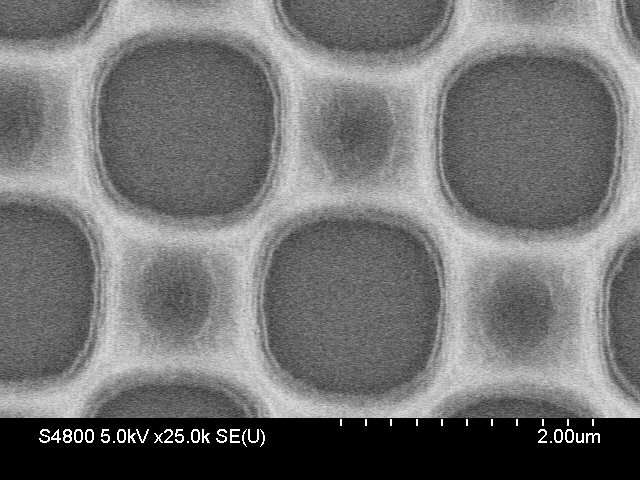
\includegraphics{data/sem/b3a10_q11.jpg}}
	\caption{For structure sizes $\sim$1 $\mu$m the patterns lose recognizability.}
	\label{fig:b2d10_q11}
\end{subfigure}
\caption{SEM images of the positive tone sample with an exposure time of 2 minutes}
\end{figure*}

The checkerboard pattern starts to decline in resolution between lengths of 2 and 10 $\mu$m. The images taken with the SEM show the same decline in resolution between 2 and 10 $\mu$m, as can be seen in the appendix.


It was found that for the negative recipe an exposure time of 0.1 minute resulted in no pattern creation at all, while exposure times of 0.5 minutes and longer resulted in overexposure of the pattern. The results of the developed samples with exposure times between 0.1 and 0.5 minutes are shown in figures \ref{fig:b2d1}, \ref{fig:b2h1} and \ref{fig:b2i1}:

\begin{figure*}[ht]
    \centering
    \begin{subfigure}[t]{0.3\linewidth}
        \centering
        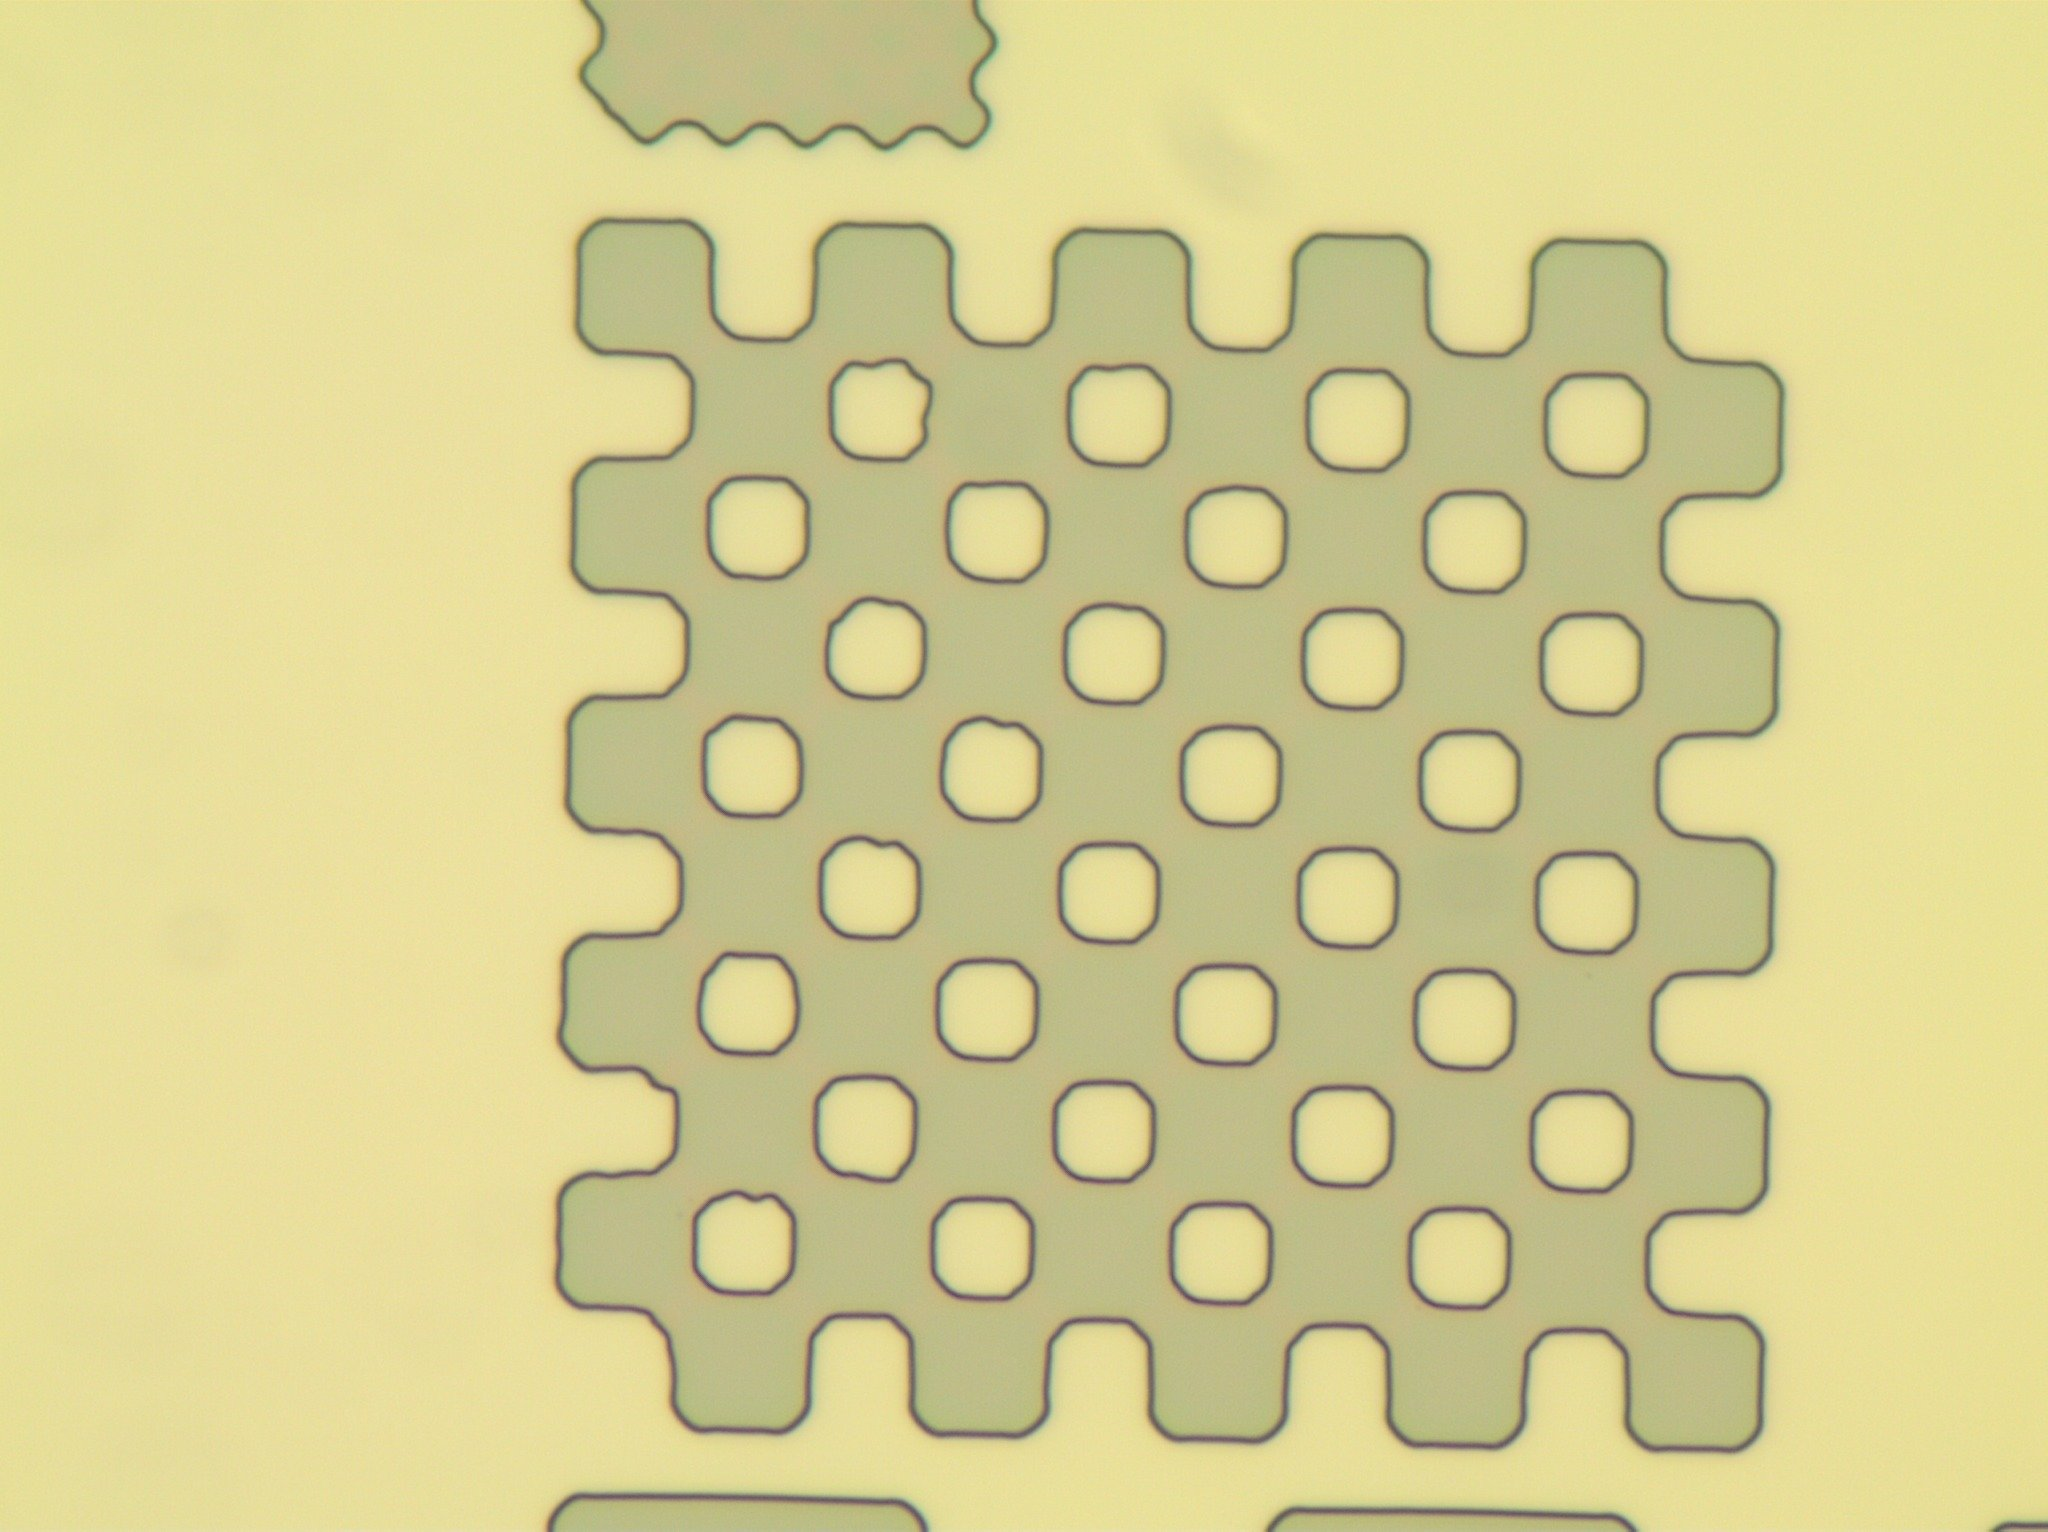
\includegraphics[width=\textwidth]{data/b2d1.jpg}
	\caption{Sample of the negative resist pattern with an exposure time of 0.5 minutes.Taking into account that a negative tone was used, it can be seen that the sample was clearly overexposed.}
	\label{fig:b2d1}
    \end{subfigure}
    \hfill
    \begin{subfigure}[t]{0.3\linewidth}
        \centering
        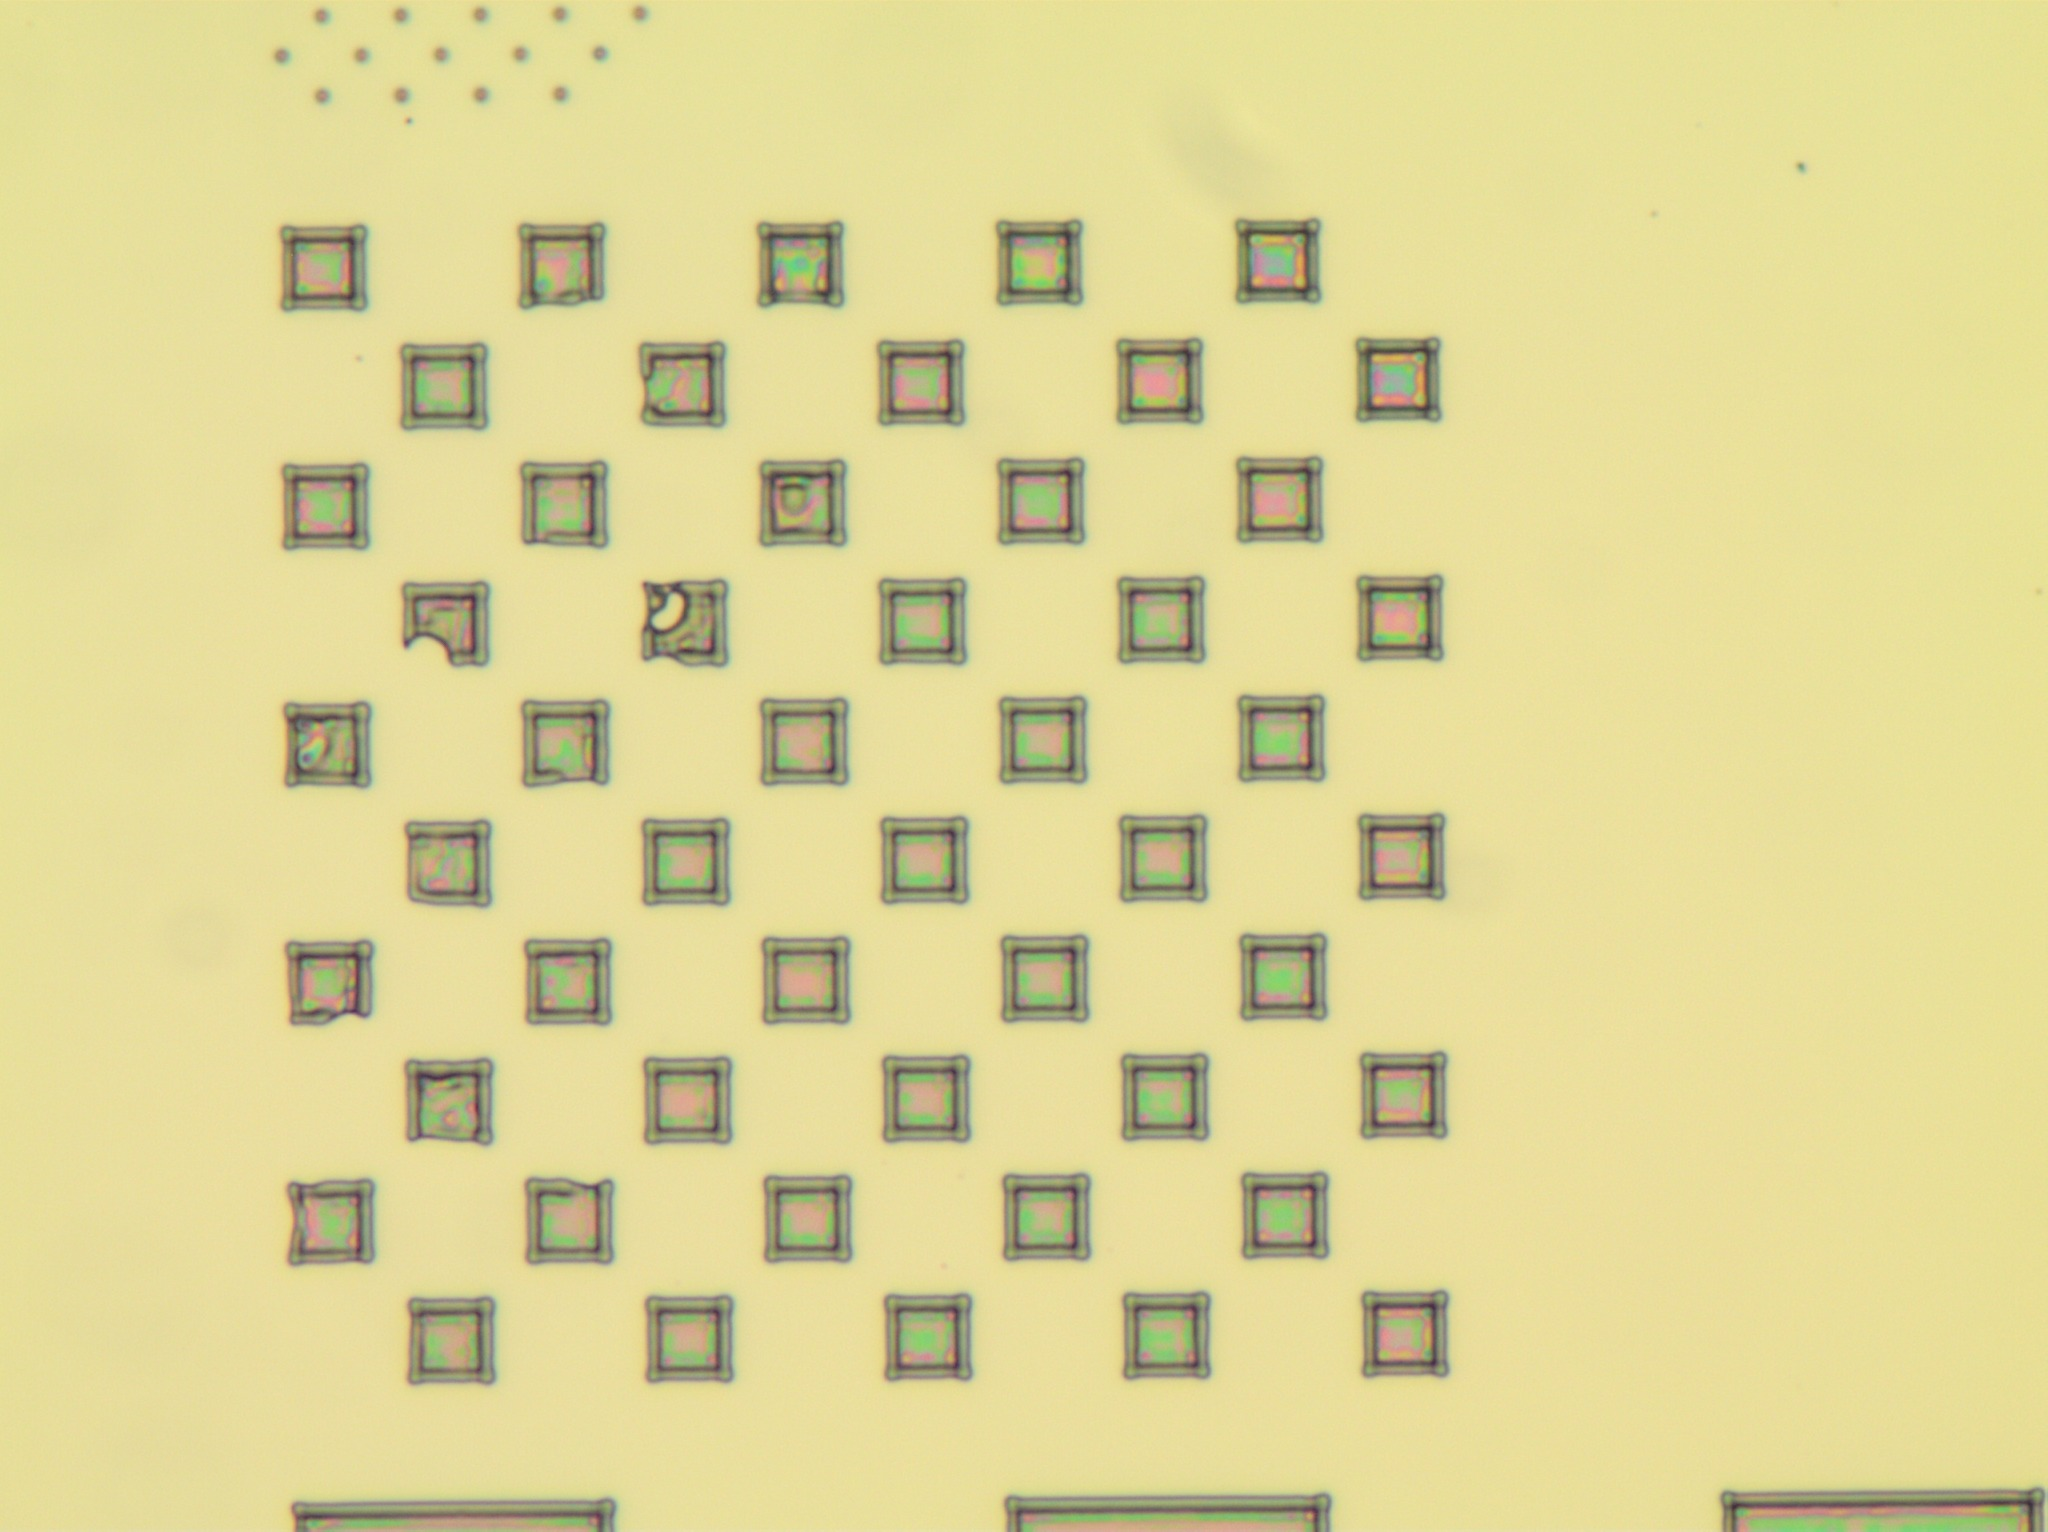
\includegraphics[width=\textwidth]{data/b2h1.jpg}
	\caption{Sample of the negative resist pattern with an exposure time of 0.2 minutes. Note that the sample is underexposed.}
	\label{fig:b2h1}
    \end{subfigure}
    \hfill
    \begin{subfigure}[t]{0.3\linewidth}
        \centering
        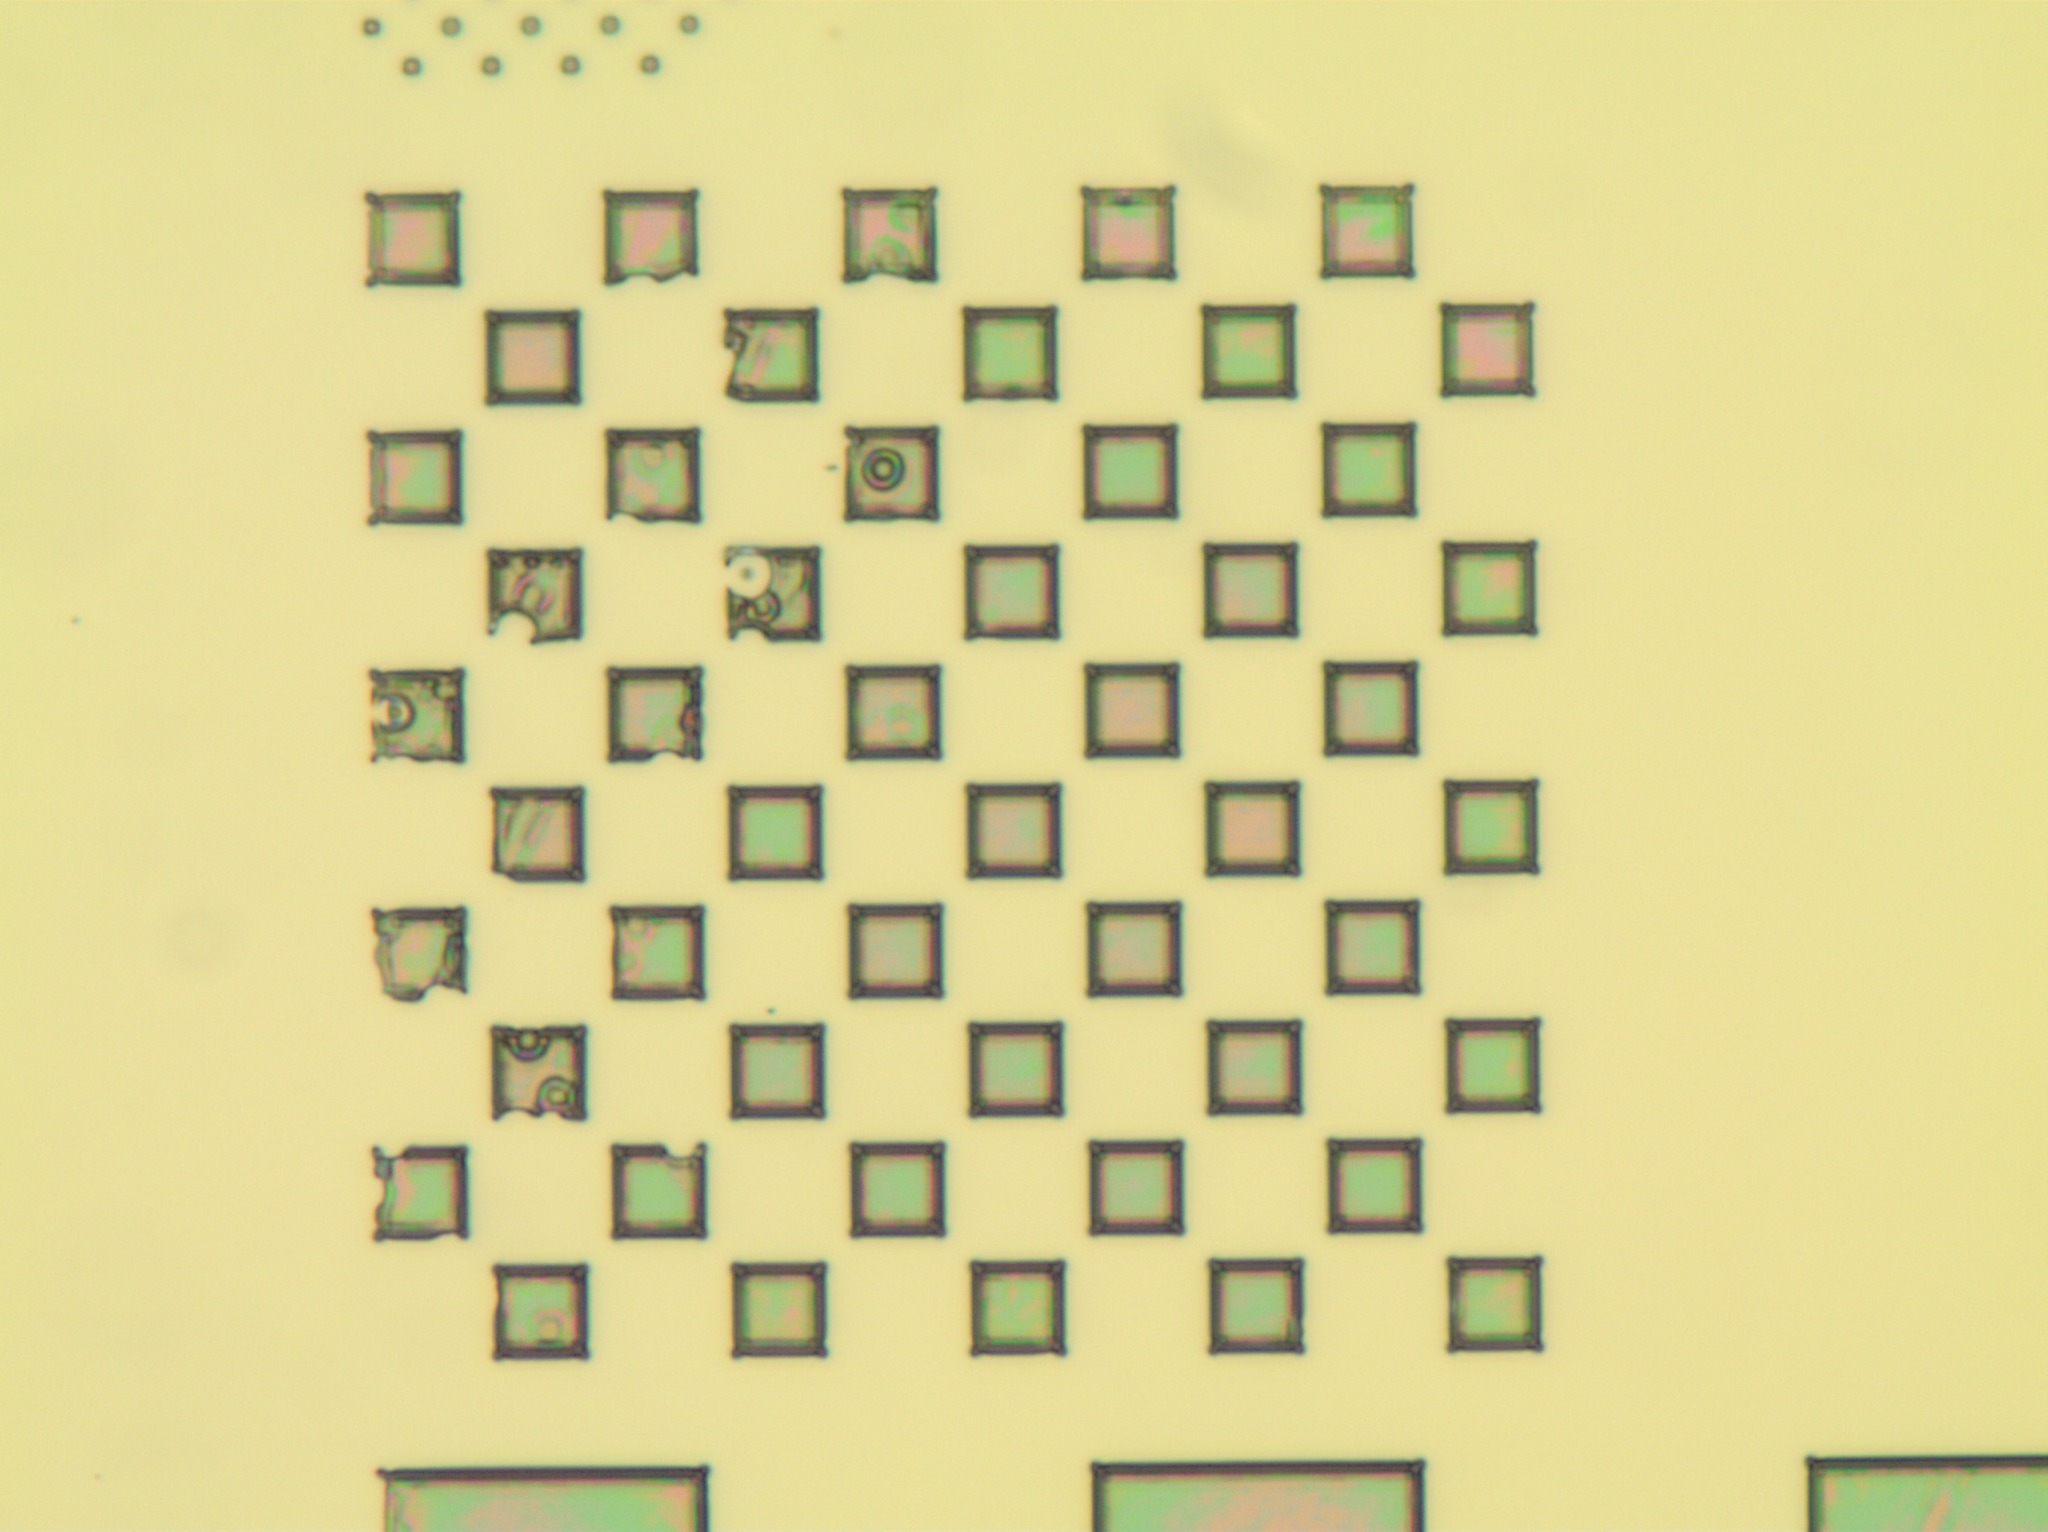
\includegraphics[width=\textwidth]{data/b2i1.jpg}
	\caption{Sample of the negative resist pattern with an exposure time of 0.3 minutes. The sample is again underexposed, but not as much as the sample with an exposure time of 0.2 minutes.}
	\label{fig:b2i1}
    \end{subfigure}
    \hfill
    % \rule{\linewidth}{3cm}
    \caption{Negative tone resist with different exposure times.}
\end{figure*}



From this we conclude that when using image reversal with the AZ~5214E an exposure time of around 0.4 minutes will be optimal for lithography. Images of the checkerboard pattern of the sample with an exposure time of 0.5 minutes under the Hitachi S4800 SEM are seen below:


\begin{figure*}[ht]
  \begin{subfigure}[t]{0.24\linewidth}
	\centering
	\resizebox{\linewidth}{!}{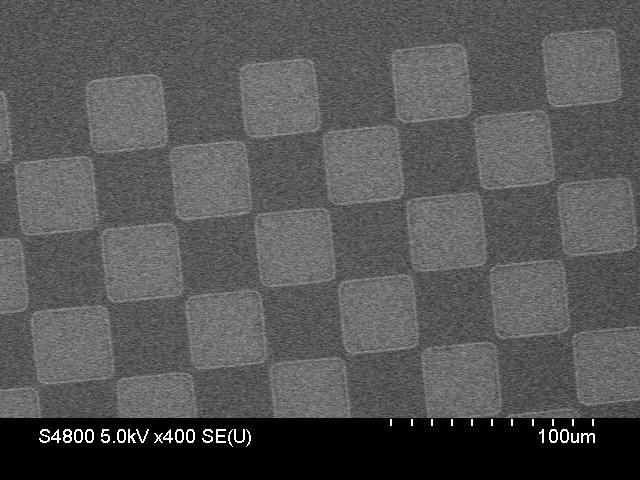
\includegraphics{data/sem/b2d26_q26.jpg}}
	\caption{SEM}
	\label{fig:b2d26_q26}
\end{subfigure}
  \begin{subfigure}[t]{0.24\linewidth}
	\centering
	\resizebox{\linewidth}{!}{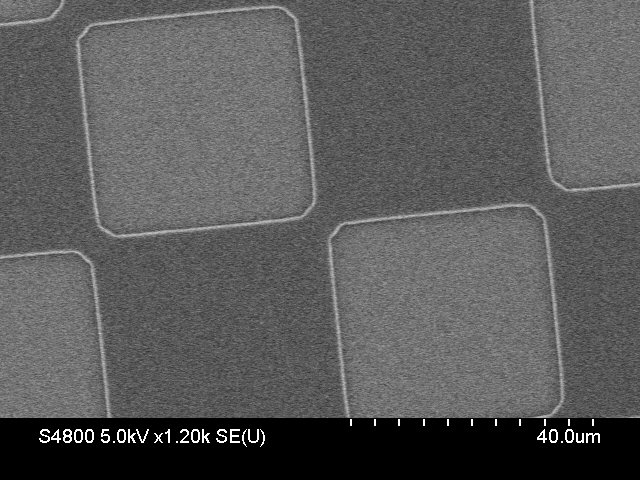
\includegraphics{data/sem/b2d27_q27.jpg}}
	\caption{SEM}
	\label{fig:b2d27_q27}
\end{subfigure}
  \begin{subfigure}[t]{0.24\linewidth}
	\centering
	\resizebox{\linewidth}{!}{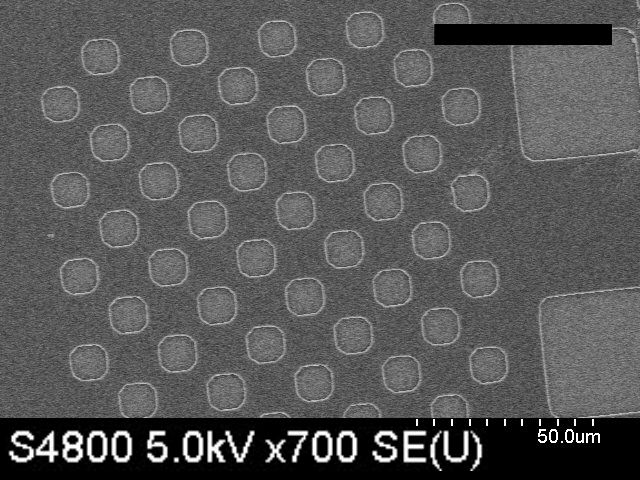
\includegraphics{data/sem/b2d28_q28.jpg}}
	\caption{SEM}
	\label{fig:b2d28_q28}
\end{subfigure}
  \begin{subfigure}[t]{0.24\linewidth}
	\centering
	\resizebox{\linewidth}{!}{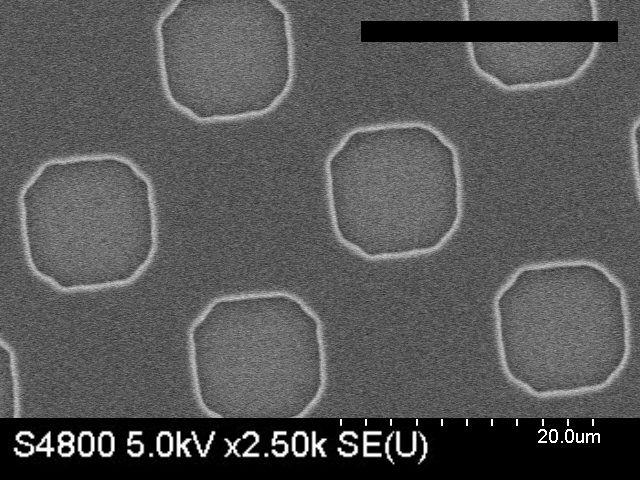
\includegraphics{data/sem/b2d29_q29.jpg}}
	\caption{SEM}
	\label{fig:b2d29_q29}
\end{subfigure}
\end{figure*}


The samples were also analyzed under a profilometer.

\begin{table}[H]
    \centering
    \caption{Positive resist thickness}
    \begin{tabular}{X l l l}
        Exp. time (min)& $\Delta h_1$ (nm)& $\Delta h_2$ (nm) \\ 
        \hline\hline
        3.0 & 1608.1  &   1578.3  \\
        4.0 & 1662.7  &   1676.4  \\
        1.0 & 320.9   &   314.0   \\
        2.5 & 1628.6  &   1628.6  \\
        3.5 & 1587.7  &   1596.2  \\
        \hline
    \end{tabular}
    \label{tab:pos_profile}
\end{table}

\begin{table}[H]
    \centering
    \caption{Negative resist thickness}
    \begin{tabular}{X l l l l}
	Exp. 1 (min) & Exp. 2(min)& $\Delta h_1$ (nm) & $\Delta h_2 (nm)$ \\ 
        \hline\hline
        0.5 & 3.0 & 1392.5  &   1376.4  \\
        1.0 & 3.0 & 1416.9  &   1547.43 \\
        1.5 & 3.0 & 1673.2  &   1690.1  \\
        0.5 & 4.0 & 1551.7  &   1522.6  \\
        1.0 & 4.0 & 1557.2  &   1547.1  \\
        1.5 & 4.0 & 1552.0  &   1524.1  \\
        0.1 & 4.0 & 45.047  &   ~       \\
        0.2 & 4.0 & 801.17  &   926.17  \\
        0.3 & 4.0 & 575.98  &   556.88  \\
        \hline
    \end{tabular}
    \label{tab:neg_profile}
\end{table}

It is clear from the table that the positive sample with an exposure time of  1 minute and the negative sample with an exposure time of 0.1 minutes almost had no activation of the photosensitive resist. No significant overcut was detected under the profilometer for the positive samples. The possible undercut was not measured for the negative samples.
While the exposure time is of importance, the development time also plays a role. During the analyzing of a batch of positive resist samples, it was found that the quality of the samples fluctuated, and that in general longer exposure times were required. 


\todo[inline]{Images of the checkerboard pattern for all samples can be found in the appendix.}